% !TEX program = xelatex
%\documentclass[10pt,letterpaper]{article}
%\usepackage{beamerarticle}
%\documentclass[notes=hide]{beamer}
\documentclass[notes=show]{beamer}

\usepackage{newtxtext}
\usepackage{bucolors}
\usepackage{analchem}
\usepackage{lecture}
\usepackage{pdfpages}
\usepackage{ccicons}

\graphicspath{{./Figures/}}

\title{Introduction to Analytical Chemistry}
\author{D.A.\ McCurry}
\institute[Bloomsburg University] % (optional)
{Department of Chemistry and Biochemistry\\
  Bloomsburg University}
\date{Fall 2021}

\begin{document}

%\mode<presentation>{
%
%\begin{frame}<handout:0>{Welcome to Analytical Chemistry I!}
%	\centering
%
%	\includegraphics[width=\linewidth]{lasvegas.png}
%\end{frame}
%}

\maketitle
\mode<article>{\thispagestyle{fancy}}

\begin{frame}
	\section{What is Analytical Chemistry?}
\end{frame}

\mode<article>{%
	Analytical chemistry deals with the
	identification and separation of materials \alert{and} the
	determination of its relative amount.

	\begin{center}
		\sffamily
		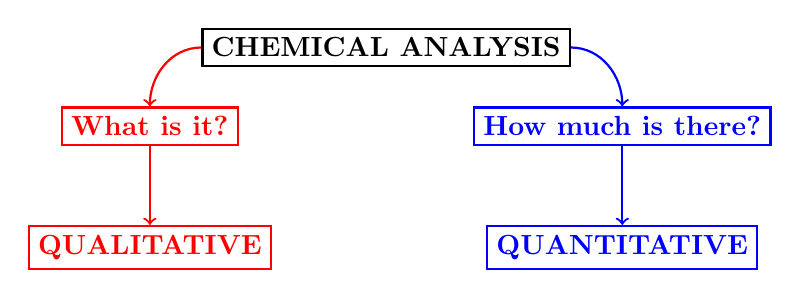
\begin{tikzpicture}
			\node[draw,thick](title) at (0,0) {\bfseries CHEMICAL
				ANALYSIS};
				\node[draw,thick,red](qual) at (-3,-1)
				{\bfseries What is it?};
				\draw[->,thick,red] (title.west) to
				[in=90,out=180] (qual.north);
				\node[draw,thick,blue](quant) at (3,-1)
				{\bfseries How much is there?};
				\draw[->,thick,blue] (title.east) to
				[in=90,out=0] (quant.north);
				\draw[->,thick,red] (qual.south) to ++(0,-1)
				node[below,draw,thick,red]{\bfseries
				QUALITATIVE};
				\draw[->,thick,blue] (quant.south) to ++(0,-1)
				node[below,draw,thick,blue]{\bfseries
				QUANTITATIVE}; 
		\end{tikzpicture}
	\end{center}
}

\begin{frame}{Why is analytical chemistry important?}
	\mode<presentation>{%
		\centering
		\includegraphics[width=\textwidth,trim={0.75in 4.25in 0.75in 1.5in},clip]{COVIDsensor.pdf}
	}
	\mode<article>{\textit{Anal. Chem.} \textbf{2020}, 92, 7226-7231}
\end{frame}

\begin{frame}{Steps in Chemical Analysis}
	\begin{center}
		\includegraphics[scale=0.7]{AnalyticalProcess.png}
	\end{center}
\end{frame}

\begin{frame}[t]
	\frametitle{The Vocabulary of Analytical Chemistry}
	\begin{itemize}
		\item Analyte
		\item Technique vs Method vs Procedure vs Protocol
		\item Accuracy vs Precision
		\item Sensitivity vs Selectivity
		\item Robust vs Rugged
		\item Reagent vs Method vs Field Blank
		\item Calibration
		\item Validation
	\end{itemize}
\end{frame}


\begin{frame}{Constructing a Representative Sample}
	\begin{itemize}
		\item Chemical analysis is meaningless if we cannot demonstrate
			that the sample is \alert{representative} of the
			population.
		\item What factors influence the validity of the data?
	\end{itemize}

	\begin{center}
		\includegraphics[width=\linewidth]{box0-1.png}
	\end{center}
\end{frame}

\begin{frame}<presentation>
	\begin{center}
		\includegraphics[width=0.8\linewidth]{RadNet-US.png}
	\end{center}
	\let\thefootnote\relax\footnotetext{\url{https://www.epa.gov/radnet/near-real-time-and-laboratory-data-state}}
\end{frame}

\begin{frame}<presentation>
	\centering
	\includegraphics[width=0.95\linewidth,page=1]{CostNews2012Nov.pdf}
\end{frame}

%\mode<article>{\includepdf[pages=1]{CostNews2012Nov.pdf}}

\begin{frame}
	\section{Chemical Measurements}
	\begin{learningobjectives}
		\item Understand common units in chemistry.
		\item Convert between different units.
		\item Use formality, molarity, and normality appropriately.
	\end{learningobjectives}
\end{frame}

\begin{frame}{Units}
	\begin{itemize}
		\item Units are \emph{very} important in analytical chemistry!

		\item Common units and terms:
	\begin{center}
	\begin{tabular} {l l c c c}
		length: & meter & \si{\meter} \\
		mass: & kilogram & \si{\kilo\gram} \\
		time: & second & \si{\second} \\
		electric current: & ampere & \si{\ampere} \\
		temperature: & kelvin & \si{\kelvin} \\
		pressure: & pascal & \si{\pascal} & \emph{or} &
			\si{\newton\per\meter\squared} \\
	\end{tabular}
	\end{center}

	\begin{block}{Syst\`{e}me International d'Unit\'{e}s (SI units)}
		see Tables 1-1, 1-2; page 12 in Harris
	\end{block}
	\end{itemize}
\end{frame}

\mode<presentation>{%
	\begin{frame}{Improper units can be catastrophic!}
		\only<1>{%
			\includegraphics[width=\linewidth]{Gimli_glider.JPG}
			
			\footnotesize By Source, Fair use,
			https://en.wikipedia.org/w/index.php?curid=18952968
		}
	
		\only<2>{\includegraphics[width=\linewidth]{MarsOrbiter.pdf}}
	\end{frame}
}

\begin{frame}{Concentrations}
	The amount of \alert{solute} dissolved in a specific amount of
	\alert{solution} or \alert{solvent}.
	\begin{align*}
		\intertext{Some common examples you have probably seen before:}
		\text{molarity (\si{\Molar})} &=
		\dfrac{\text{\si{\mole}~solute}} {\text{\si{\liter}~solution}}
		\\
		\text{molality (\si{\molal})} &=
		\dfrac{\text{\si{\mole}~solute}}
		{\text{\si{\kilo\gram}~solvent}}
		\visible<2>{
		\intertext{And some you might not have:}
		\text{formality (\si{\formal})} &=
		\dfrac{\text{\si{\mole}~\alert{ionic~compounds}}}
		{\text{\si{\liter}~solution}} \\
		\text{normality (\si{\normal})} &= \dfrac{\text{reactive
		\alert{equivalents}}}{\text{\si{\liter}~solution}}
		}
	\end{align*}
\end{frame}

\begin{frame}{Why bother with formality?}
	\mode<presentation>{
	\only<1>{\begin{center}
		\includegraphics[width=\linewidth]{formality-scale.png}
	\end{center}
	}}

	\only<2->{
		\begin{itemize}[<+(1)->]
		\item Long answer: it is more reflective of the actual
			concentration of the species present in solution
			\begin{itemize}
				\item Strong electrolytes dissociate completely
					in solution:
					\begin{reaction*}
						!(\SI{1}{\formal})(NaCl) ->[ H2O
						] !(\SI{1}{\Molar})( Na+ ) +
						!(\SI{1}{\Molar})( Cl- )
					\end{reaction*}
				\item Weak electrolytes do not dissociate
					completely in solution:
					\begin{reaction*}
						!(\SI{1}{\formal})( HF ) <=>[ H2O ]
						!(\SI{<1}{\Molar})( H+ ) +
						!(\SI{<1}{\Molar})( F- )
					\end{reaction*}
			\end{itemize}
		\item Short answer: most often we don't --- it is widely understood that molarity $\equiv$ formality.
	\end{itemize}
}
\end{frame}

\begin{frame}{Why bother with normality?}
	\begin{itemize}
		\item For some reactions, it may be more convenient to consider
			the \alert{reactive equivalents} offered by a reactant
		\item In particular, \alert{acid-base titrations} can be a bit
			simpler to think of in terms of normality

			\begin{center}
				\ch{H2SO4 + 2 NaOH -> Na2SO4 + 2 H2O}
			\end{center}

			\emph{Both} \ch{H+} in \ch{H2SO4} will react with
			\ch{OH-} to produce 2 \emph{equivalents} of \ch{H2O}
			\begin{align*}
				\therefore \SI{1}{\Molar}~\ch{H2SO4} &=
				\SI{2}{\normal}~\ch{H2SO4}
			\end{align*}
	\end{itemize}
\end{frame}

\begin{frame}[t]{Conversions}
	A concentrated HF solution is \SI{48.1}{\percent} by weight \ch{HF} and
	has a density of \SI{1.15}{\gram\per\milli\liter}. What are the formal
	and molal concentrations of \ch{HF}?

	\mode<article>{\vspace{15em}}

\note<+>{
	\begin{enumerate}
		\item Assume \SI{100.0}{\gram}~solution $\therefore$
			\SI{48.1}{\gram}~HF and \SI{51.9}{\gram}~\ch{H2O}
		\item Calculate moles HF: \SI{2.393}{\mole}~\ch{HF}
		\item This is enough to provide molality:
			\begin{align*}
				\dfrac{\SI{2.393}{\mole}~\ch{HF}}
				{\SI{0.0519}{\kilo\gram}~\text{solvent}}
				= \SI{46.1}{\molal}~\ch{HF}
			\end{align*}
		\item Use density to find volume of solution:
			\begin{align*}
				\SI{100.0}{\gram}~\text{solution} \times
				\dfrac{\SI{0.001}{\liter}}{\SI{1.15}{\gram}} =
				\SI{0.08696}{\liter}
			\end{align*}
		\item Calculate formality:
			\begin{align*}
				\dfrac{\SI{2.393}{\mole}}{\SI{0.08696}{\liter}}
				= \SI{27.5}{\formal}~\ch{HF}
			\end{align*}
	\end{enumerate}
}
\end{frame}

\begin{frame}[t]{Exponent Removal}
	The concentration of barium ion in a produced water sample was found to
	be \SI{2.51e-7}{\Molar}.

	\begin{itemize}[<+->]
		\item Prefixes (kilo, milli, centi, \ldots)
			\only<.>{%
				\begin{align*}
					\SI{2.51e-7}{\Molar} =
					\dfrac{\SI{2.51e-7}{\mole}}{\si{\liter}}
					\times
					\dfrac{\SI{e6}{\micro\mole}}{\SI{1}{\mole}} =
					\SI{0.251}{\micro\Molar}
				\end{align*}
			}
		\item p-function: $\p{\ch{X}} = -\log [\ch{X}]$
			\only<.>{%
				\begin{align*}
					\p{\ch{Ba}} = -\log(\num{2.51e-7}) = 6.600
				\end{align*}
			}
		\item parts-per-concentrations (ppm, ppb, ppt, \ldots)
			\only<.>{%
				\begin{align*}
					\SI{2.51e-7}{\Molar} \times
					\SI{137327}{\milli\gram\per\mole}~\ch{Ba} &=
					\SI{0.0344}{\milli\gram\per\liter}~\ch{Ba^{2+}}
					\\
					&= \SI{0.0344}{ppm}\footnotemark[1]~\ch{Ba^{2+}} \\
					&= \SI{34.4}{ppb}\footnotemark[1]~\ch{Ba^{2+}}
				\end{align*}

				\bigskip
				\footnotetext[1]{Only in water ($d = \SI{1.00}{\gram\per\milli\liter}$), ppm = mg/L;
			ppb = \si{\micro\gram}/L;  ppt = ng/L.}
			}
	\end{itemize}
\end{frame}

\begin{frame}{Why is \SI{1}{\milli\gram\per\liter} = \SI{1}{ppm}?}

	\mode<article>{\vspace{15em}}

\note{
	\begin{align*}
		\text{ppm} &= \dfrac{\SI{1}{part}}{\SI[inter-unit-product={ }]{1}{million~parts}} =
			\dfrac{\SI{1}{part}}{\SI{e6}{parts}} \\
			\shortintertext{}
		d_{\ch{H2O}} &= \dfrac{\SI{1}{\gram}}{\SI{1}{\milli\liter}} =
		\dfrac{\SI{1}{\gram}}{\SI{e-3}{\liter}} \times
		\dfrac{\SI{1}{\milli\gram}}{\SI{0.001}{\gram}} =
		\dfrac{\SI{1}{\milli\gram}}{\SI{e-6}{\liter}} =
		\SI{e6}{\milli\gram\per\liter}\\
	\end{align*}

	$\therefore$ in \SI{1}{\liter}~\ch{H2O}, we have
\SI{e6}{\milli\gram}~\ch{H2O}, or ``\SI[inter-unit-product={ }]{1}{million~parts}''.}
\end{frame}

\begin{frame}[t]{Problem}
	A pesticide (\SI{408.8}{amu}) is extracted from a \SI{1.000}{\liter}
	ground water sample into \SI{25.00}{\milli\liter} of hexane. GC
	analysis indicates the latter solution contains \SI{52.1}{ppb}
	pesticide. What is the molar concentration in the original ground
	water?

	\pause

	\begin{center}
		(The density of hexane is \SI{0.6548}{\gram\per\milli\liter})
	\end{center}

	\mode<article>{\vspace{15em}}

\note<+>{
	\begin{align*}
		\si{ppb} &= \dfrac{\text{mass of substance}}{\text{mass of sample}} \times \num{e9} \\
	\text{mass of sample}  &= \SI{25.00}{\milli\liter}~\text{hexane} \times \dfrac{\SI{0.6548}{\gram}}{\SI{1}{\milli\liter}} = \SI{16.37}{\gram}~\text{hexane} \\
\SI{52.1}{ppb} &= \dfrac{x}{\SI{16.37}{\gram}} \times \num{e9} \therefore x = \SI{8.529e-7}{\gram}~\text{pesticide} \\
		& \SI{8.529e-7}{\gram}~\text{pesticide} \times \dfrac{\SI{1}{\mole}}{\SI{408.8}{\gram}} = \SI{2.086e-9}{\mole} \\
		& \therefore \fbox{\SI{2.09e-9}{\Molar} or \SI{2.09}{\nano\Molar}}
	\end{align*}
	}
\end{frame}

\frame{\section{Dilutions}
	\begin{learningobjectives}
		\item Calculate a new concentration provided volumes and an initial concentration.
		\item Determine what volumes you will need to use in order to prepare a solution of a specific
			concentration.
		\item Determine the original concentration of an unknown solution that you had previously diluted.
	\end{learningobjectives}
}

\begin{frame}[t]{Dilutions}
	\begin{align*}
		M_\text{conc} V_\text{conc} = M_\text{dil} V_\text{dil}
	\end{align*}

	How would you prepare a liter of \SI{0.200}{\formal}~\ch{HCl} from
	\SI{11.8}{\formal} stock?

	\pause

	\mode<presentation>{\vskip0pt plus 1filll}
	\mode<article>{\vspace{15em}}

	\begin{block}{Lab Technique:}
		Transfer $V_\text{conc}$ concentrated \ch{HCl} to a
		\SI{1.00}{\liter} volumetric flask and dilute to volume. Shake
		well at intermediate and final volume.
	\end{block}

	\note<.>{
	\begin{align*}
		(\SI{11.8}{\formal})(V_\text{conc}) &=
		(\SI{0.200}{\formal})(\SI{1.00}{\liter}) \\
		V_\text{conc} &=
		\dfrac{(\SI{0.200}{\formal})(\SI{1.00}{\liter})}{\SI{11.8}{\formal}} \\
		V_\text{conc} &= \SI{17.0}{\milli\liter}
	\end{align*}
	}
\end{frame}

\end{document}
		
